\documentclass[]{report}

\voffset=-1.5cm
\oddsidemargin=0.0cm
\textwidth = 480pt

\usepackage{framed}
\usepackage{subfiles}
\usepackage{enumerate}
\usepackage{graphics}
\usepackage{newlfont}
\usepackage{eurosym}
\usepackage{amsmath,amsthm,amsfonts}
\usepackage{amsmath}
\usepackage{color}
\usepackage{amssymb}
\usepackage{multicol}
\usepackage[dvipsnames]{xcolor}
\usepackage{graphicx}
\begin{document}
\chapter{Set theory}
\section*{Set Theory}

\begin{itemize}
\item[1.1] Introduction  
\item[1.2] Sets  
\item[1.3] Sub-sets  
\item[1.4] The order of sets: finite and infinite sets .
\item[1.5] Union and intersection of sets  
\item[1.6] Differences and complements  
\item[1.7] Venn diagrams  
\item[1.8] Logic analysis
\end{itemize}  
%-----------------------------------------------------%
\newpage
\subsection*{Union and intersection of sets}

\begin{itemize}
\item The \textbf{union} of two sets A and B is a set containing all the elements in
either A or B (or both)
i.e. 
\[A \cup B = {x / x \in A \mbox{ or } x \in B}.\]
\item The \textbf{intersection} of two sets A and B is a set containing all the elements
that are both in A and B
i.e. 
\[A \cap B = {x / x \in A \mbox{ and }x \in B}\].

\item If sets A and B have no elements in common, i.e. $A \cap B = \emptyset$,then A and B
are termed \textbf{disjoint sets}.
\end{itemize}

\subsection*{Subsets}

\begin{itemize}
\item Proper Subsets
\end{itemize}
\subsection*{The Power Set}


% Ex 2
\section{Video 2 : Set Theory}
%--------------------------------------------%

%\frametitle{Set Theory : Set Operations}

Given the following sets

\begin{center}
\begin{tabular}{|c|c|} \hline
$\mathcal{U}$ & $\{1,2,3,4,5,6,7,8,9\}$ \\ \hline
$\mathcal{A}$ & $\{1,2,5,6,8\}$ \\ \hline
$\mathcal{B}$ & $\{3,5,7,8\}$ \\ \hline
$\mathcal{C}$ & $\{5,6,7,8,9\}$ \\ \hline
\end{tabular}
\end{center}

List the elements of the following
$A^{\prime} \cap B $\\
$A^{\prime} \cap C $\\

%--------------------------------------------%

\section*{Venn Diagrams}

Subsets of the universal set $\mathcal{U}$, intersecting in the most general way (Essentially this means - the venn diagram allows for all possible combinations of overlap.)

\begin{center}
\begin{tabular}{|c|c|}
\hline  &  \\ 
\hline  &  \\ 
\hline 
\end{tabular} 
\end{center}

%-------------------------- %
%-------------------------- %
%Section 3

\section*{Question 2}
HibCollWorkSheet2

%Listing Method
%Rules of Inclusion
%Cardinality
%Venn diagrams

$\in$
$\subset$

univeral Set $\mathcal{U}$
Laws for Binary Operations
Membership Tables

De Morgan's Law


\[A^{\prime} \cup B^{\prime} = A \cap B\]

\subsection*{Part A : Builder Method}
The following sets have been defined using the \textbf{Building Method} of notation. Re-write them by listing \textbf{some} of the elements.
\begin{enumerate}
\item $\{p | p$ is a capital city, p is in Europe$\}$
\item $\{x | x = 2n - 5,$ x and n are natural numbers$\}$
\item $\{y | 2y^2 = 50,$ y is an integer$\}$
\item $\{z | z = n^3,$ z and n are natural numbers$\}$
\end{enumerate}
\subsection*{Part B : Sets}
U = {natural numbers}; $A = \{2, 4, 6, 8, 10\}$; $B = \{1, 3, 6, 7, 8\}$. State whether each of the following is true or false:
\begin{itemize}
\item[(i)] $A \subset U$
\item[(ii)] $B \subseteq A$
\item[(iii)] $\emptyset \subset U$
\end{itemize}

%-------------------------------------- %

\section*{Question 2}
\subsection*{Part A : Builder Method}
The following sets have been defined using the \textbf{Building Method} of notation. Re-write them by listing \textbf{some} of the elements.
\begin{enumerate}
\item $\{p | p$ is a capital city, p is in Europe$\}$
\item $\{x | x = 2n - 5,$ x and n are natural numbers$\}$
\item $\{y | 2y^2 = 50,$ y is an integer$\}$
\item $\{z | z = n^3,$ z and n are natural numbers$\}$
\end{enumerate}
\subsection*{Part B : Sets}
U = {natural numbers}; $A = \{2, 4, 6, 8, 10\}$; $B = \{1, 3, 6, 7, 8\}$. State whether each of the following is true or false:
\begin{itemize}
\item[(i)] $A \subset U$
\item[(ii)] $B \subseteq A$
\item[(iii)] $\emptyset \subset U$
\end{itemize}

%-------------------------------------- %

%--------------------------------------------------------%
\subsubsection*{Relative Difference}
\begin{itemize}
\item $ A \otimes B$
\end{itemize}
%--------------------------------------------------------%
\subsubsection*{Power Sets}
\begin{itemize}
\item Consider the set A where $ A = \{w,x,y,z\}$
\item There are 4 elements in set A.
\item The power set of A contains 16 element data sets.
\item \[  \mathcal{P}(A) = \{\{ x \}, \{ y \} \}  \]
\item (i.e. 1 null set, 4 single element sets, 6 two -elemnts sets, 4 three lement set and one 4- element set.)
\end{itemize}
%------------------------------------------------%
\newpage
\begin{itemize}
\item $ p \rightarrow q$  p implies q
\item $p \lg q $
\end{itemize}
\newpage

%--------------------------------------------------------%
\subsubsection*{Relative Difference}
\begin{itemize}
\item $ A \otimes B$
\end{itemize}
%--------------------------------------------------------%
\subsubsection*{Power Sets}
\begin{itemize}
\item Consider the set A where $ A = \{w,x,y,z\}$
\item There are 4 elements in set A.
\item The power set of A contains 16 element data sets.
\item \[  \mathcal{P}(A) = \{\{ x \}, \{ y \} \}  \]
\item (i.e. 1 null set, 4 single element sets, 6 two -elemnts sets, 4 three lement set and one 4- element set.)
\end{itemize}
%------------------------------------------------%
\newpage
\begin{itemize}
\item $ p \rightarrow q$  p implies q
\item $p \lg q $
\end{itemize}
%---------------------------- %
%---------------------------------------%
\subsection*{Dice Rolls}
Consider rolls of a die. What is the universal set?

\[ \mathcal{U} = \{1,2,3,4,5,6\} \]

%--------------------------------------%
\subsection*{Worked Example}

Suppose that the Universal Set $\mathcal{U}$ is the set of integers from 1 to 9.
\[ \mathcal{U} = \{1,2,3,4,5,6,7,8,9\}, \]

and that the set $\mathcal{A}$ contains the prime numbers between 1 to 9 inclusive.

\[ \mathcal{A} = \{1,2,3,5,7\}, \]

and that the set $\mathcal{B}$ contains the even numbers between 1 to 9 inclusive.

\[ \mathcal{B} = \{2,4,6,8\}. \]

%--------------------------------------------------------%
\subsubsection*{Complements}
\begin{itemize}

\item The Complements of A and B are the elements of the universal set not contained in A and B.

\item The complements are denoted $\mathcal{A}^{\prime}$ and $\mathcal{B}^{\prime}$
\[ \mathcal{A}^{\prime} = \{4,6,8,9\}, \]
\[ \mathcal{B}^{\prime} = \{1,3,5,7,9\}, \]

\end{itemize}


%--------------------------------------------------------%

\subsubsection*{Intersection}
\begin{itemize}

\item Intersection of two sets describes the elements that are members of both the specified Sets

\item The intersection is denoted $\mathcal{A\cap B}$ 
\[ \mathcal{A\cap B} = \{2\}\]

\item only one element is a member of both A and B.
\end{itemize}
%--------------------------------------------------------%

\subsubsection*{Set Difference}
\begin{itemize}

\item The Set Difference of A with regard to B are list of elements of A not contained by B.

\item The complements are denoted $\mathcal{A-B}$ and $\mathcal{B-A}$
\[ \mathcal{A-B} = \{1,3,5,7\}, \]

\[ \mathcal{B-A} = \{4,6,8\}, \]
\end{itemize}
\subsection*{symbols}
$\varnothing$,
$\forall$,
$\in$,
$\notin$,
$\cup$
%----------------------------------------------------------- %


%------------------------------------------$

\subsection*{2008  Zone A question2a}
$B = \{3n-1 :n \in Z^{+} \}$
Describe the set B using the listing method

\begin{itemize}
\item Let $n=1$. Consequently $3(1)-1 =2$
\item Let $n=2$. Likewise $3(2)-1 =5$
\item Let $n=3$. $3(3)-1 = 8 $
\item The repeated differences are 3. The next few values are 11, 14 and 17
\item So by the listing method $B= \{2,5,8,11,14,17,\ldots\}$
\end{itemize}

$A = \{3,5,7,9,ldots \}$
Describe the set A using the rules of inclusion method

\begin{itemize}
\item The repeated differences are 2.
\item We can say the rule has the form $2n+k$
\item For the first value n=1. Therefore $2+k=3$
\item Checking this , for the second value , n=2. Therefore $4+k=5$
\item Clearly k = 1.
\item $A = \{2n+1 :n \in Z^{+} \}$
\item So by the listing method $B= \{2,5,8,11,14,17,\ldots\}$
\end{itemize}

\subsection{Cartesian Product}
{
\begin{itemize}
\item Let $X$ and $Y$ be sets.
\item The \textbf{cartesian product} $X \times Y$ is the set whose elements are \textbf{all} of 
the ordered pairs of elements $(x,y)$ where $x \in X$ and $y \in Y$.
\end{itemize}

\begin{itemize}
\item Let $X = \{a,b,c\}$
\item Let $Y = \{0,1\}$ 
\item The cartesian product $X \times Y$ is therefore:
\end{itemize}

\begin{itemize}
\item Importantly $X \times Y \neq Y \times X$
\item Recall: Let $X = \{a,b,c\}$ and let $Y = \{0,1\}$ 
\item The cartesian product $Y \times X$ is therefore:
\end{itemize}
}





\subsection{The Cartesian Product}
Exercises


 Discrete Maths
 
A binary relation on a set A is the collection of ordered pairs of elements of A. In other words, it is the subset of the cartesian product A2= AA

Cartesian Product
 
This is a direct product pf 2 sets
 
XY = {(x,y)| xXandyY }
 
4 suits of cards and 13 Ranks, therefore 52 element cartesian prodcut.
 
N.B         AB BA
              A=A =
 
Cartesian product is not associative
\subsection*{Worked Example}

Suppose that the Universal Set $\mathcal{U}$ is the set of integers from 1 to 9.
\[ \mathcal{U} = \{1,2,3,4,5,6,7,8,9\}, \]

and that the set $\mathcal{A}$ contains the prime numbers between 1 to 9 inclusive.

\[ \mathcal{A} = \{1,2,3,5,7\}, \]

and that the set $\mathcal{B}$ contains the even numbers between 1 to 9 inclusive.

\[ \mathcal{B} = \{2,4,6,8\}. \]

%--------------------------------------------------------%
\subsubsection*{Complements}
\begin{itemize}

\item The Complements of A and B are the elements of the universal set not contained in A and B.

\item The complements are denoted $\mathcal{A}^{\prime}$ and $\mathcal{B}^{\prime}$
\[ \mathcal{A}^{\prime} = \{4,6,8,9\}, \]
\[ \mathcal{B}^{\prime} = \{1,3,5,7,9\}, \]

\end{itemize}


%--------------------------------------------------------%

\subsubsection*{Intersection}
\begin{itemize}

\item Intersection of two sets describes the elements that are members of both the specified Sets

\item The intersection is denoted $\mathcal{A\cap B}$ 
\[ \mathcal{A\cap B} = \{2\}\]

\item only one element is a member of both A and B.
\end{itemize}
%--------------------------------------------------------%

\subsubsection*{Set Difference}
\begin{itemize}

\item The Set Difference of A with regard to B are list of elements of A not contained by B.

\item The complements are denoted $\mathcal{A-B}$ and $\mathcal{B-A}$
\[ \mathcal{A-B} = \{1,3,5,7\}, \]

\[ \mathcal{B-A} = \{4,6,8\}, \]
\end{itemize}


\end{document}
\section*{Question 2}
Describe the following set by the rules of inclusion method.

Describe the following set by the listing method
the set of positive multiples of 3 which are less than 20.

Let A and B be subsets of univerisal set U

Use the membership rule to prove that

\[(A^\prime  \cap B)^\prime = A \cup B^\prime\]

shade the region corresponding to this set on a Venn Diagram

Given the universal set $\mathcal{U} = {1,2,3,4,5,6,7,8,9}$
and the subsets $A=\{1,3,5,7\}$
$B = \{6,7,8,9\}$
list the set $A^\prime \cap B)^\prime$ 



\begin{itemize}
\item[(i)] $\{5,8\}$
\item[(ii)] $\{1,2,3,4,5,6,7,8,9\}$ 
\end{itemize}

\section*{Set Operations}
\begin{itemize}
\item Union ($\cup$) - also known as the \textbf{OR} operator. A union signifies a bringing together. The union of the sets A and B consists of the elements that are in either A or B.
\item Intersection ($\cap$) - also known as the \textbf{AND} operator. An intersection is where two things meet. The intersection of the sets A and B consists of the elements that in both A and B.
\item Complement ($A^{\prime}$ or $A^{c}$) - The complement of the set A consists of all of the elements in the universal set that are not elements of A.
\end{itemize}

\subsection*{Exercise}
Consider the universal set $U$ such that
\[U=\{1,2,3,4,5,6,7,8,9\} \] 
and the sets
\[A=\{2,5,7,9\} \] 
\[B=\{2,4,6,8,9\} \]

\begin{multicols}{2}
\begin{itemize}
\item[(a)] $A-B$
\item[(b)] $A \otimes B$
\item[(c)] $A \cap B$
\item[(d)] $A \cup B$
\item[(e)] $A^{\prime} \cap B^{\prime}$
\item[(f)] $A^{\prime} \cup B^{\prime}$
\end{itemize}
\end{multicols}

%======================================================================================= %
\newpage

\section*{Venn Diagrams}

Draw a Venn Diagram to represent the universal set
$\mathcal{U} = \{0,1,2,3,4,5,6\}$ with subsets:\\
$A = \{2,4,5\}$\\
$B = \{1,4,5,6\}$\\

\noindent Find each of the following
\begin{itemize}
\item[(a)] $A \cup B $
\item[(b)] $A \cap B $
\item[(c)] $A-B$
\item[(d)] $B-A$
\item[(e)] $A \otimes B$
\end{itemize}
\newpage



%------------------------------------------------------------------------%
\begin{itemize}
\item[(i)] Describe the following set by the listing method
\[ \{ 2r+1 : r \in Z^{+} and r \leq 5  \} \]
\item[(ii)] Let A,B be subsets of the universal set U.


\end{itemize}

%===================================================================================== %
\subsection*{Question 1}

\begin{itemize}
\item $\{ s :  \mbox{ s is an odd integer and } 2 \leq s \leq 10 \}$
\item $\{ 2m :  m \in Z \mbox{ and }5 \leq m \leq 10 \}$
\item $\{ 2^t :  t \in Z \mbox{ and } 0 \leq t \leq 5 \}$
\end{itemize}

%=======================+============================================================== %
\subsection*{Question 2}

\begin{itemize}
\item $\{12,13,14,15,16,17\}$
\item $\{0,5,-5,10,-10,15,-15,.....\}$
\item $\{6,8,10,12,14,16,18\}$
\end{itemize}

\subsection*{Question 7 : Membership Tables}
Using membership tables
\begin{tabular}{|ccc|c|c|c|}
\hline
% after \\: \hline or \cline{col1-col2} \cline{col3-col4} ...
A & B & C & x & y & z \\\hline
0 & 0 & 0 & 1 & 1 & 1 \\
0 & 0 & 1 & 0 & 0 & 1 \\
0 & 1 & 0 & 0 & 0 & 1 \\
0 & 1 & 1 & 0 & 0 & 1 \\
1 & 0 & 0 & 1 & 0 & 1 \\
1 & 0 & 1 & 1 & 0 & 1 \\
1 & 1 & 0 & 0 & 0 & 1 \\
1 & 1 & 1 & 1 & 0 & 1 \\
\hline
\end{tabular}
\begin{itemize}
\item[(i)] Draw a venn diagram to show three subsets A,B and C of a universal set U intersecting in
the most general way?
\item[(ii)] How are sets $X$ and $Z$ related?
\item[(iii)] Can you describe each of the subsets X,Y and Z in terms  of the
sets A,B,C using the operations union intersection and set complement.
\end{itemize}
%================================================================ %
%Exercise 3
\section{Set Theory}
%--------------------------------------------%

%\frametitle{Set Theory : Set Operations}

\begin{itemize}
\item[\textbf{A}] $ \{ 2n : n \in \mathbb{Z^{+}} \} $
\item[\textbf{B}] $ \{ 3,6,9,12,15,18,\ldots \} $
\end{itemize}
\textbf{Questions}
\begin{itemize}
\item[(i)] \textbf{A} is described by the rules of inclusion. Describe \textbf{A} with the listing method.
\item[(ii)] \textbf{B} is described by the listing method. Describe \textbf{B} with the rules of inclusion. 
\end{itemize}




%------------------------------------%
\section*{Question 4}
\[ \mbox{Log}_4 64 + \mbox{Log}_5 625 + \mbox{Log}_9 3 \] 


%------------------------------------%
\section*{Question 5}
\begin{enumerate}
\item Draw two non-isomorphic graphs with the following degree sequence.
\[ 4,3,3,2,2,2,2,1,1\]
\item
\end{enumerate}
%------------------------------------%

\section*{Question 7b}

Compute the following summation

\[ \sum^{i=100}_{i=25} i^2 + 3i -5)\]


%------------------------------------%

\section*{Section 2. Set Theory}

\begin{enumerate}
\item
\item
\item
\end{enumerate}
\subsection*{Membership Tables}
For the following venn diagrams, complete the membership.

The events $W$, $X$,$Y$ and $Z$ correspond to the shaded areas in each of the venn diagrams.

%----------------------------------------- %
%----------------------------------------- %

\subsection*{Venn Diagrams}
%\begin{figure}
%\centering
%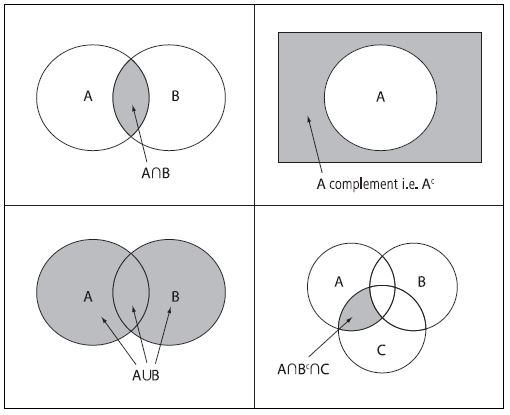
\includegraphics[width=0.7\linewidth]{venndiagram}
%
%\end{figure}
\[ \mbox{IMAGE}\]

%----------------------------------------%
%------------------------------------------------------------------------%

\section{Specifying Sets (2.1)}

\begin{enumerate}
\item Listing Method
\item Rules of Inclusion
\end{enumerate}

%------------------------------------------------------------------------%

\section{Subsets and the Power Set} (2.2)
Subsets and Proper Subsets
Cardinality of a Set
Power Set


%------------------------------------------------------------------------%

\section{Set operations (2.3)}

complement
union 
intersection
set difference


\section{Venn Diagrams}

venn diagrams
8 Disjoint Regions

%------------------------------------------------------------------------%
\section{Sets of Numbers}

\begin{itemize}
\item $\mathbb{Z}$ Set of all integers
\item $\mathbb{Q}$ Set of all rational numbers
\item $\mathbb{R}$ Set of all real numbers
\end{itemize}


\begin{itemize}
\item $\mathbb{Z}^{+}$ Set of all positive integers
\item $\mathbb{Z}^{-}$ Set of all negative integers
\item $\mathbb{R}^{+}$ Set of all positive real numbers
\item $\mathbb{R}^{-}$ Set of all negative real numbers
\end{itemize}

%------------------------------------------------------------------------%
\end{document}
